\documentclass[letterpaper,headings=standardclasses]{scrartcl}

\usepackage[margin=1in,includefoot]{geometry}
\usepackage{graphicx}
\usepackage{float}

\title{Homework 1}
\subtitle{CS 478 - Software Development for Mobile Platforms - Fall 2019}
\author{Matteo Corain 650088272}

\begin{document}

\maketitle

\section{Question 1}

In order to be able to build and run Android applications through the AVD emulator, three components are needed for each API level we want to target: the \emph{Android SDK}, the \emph{Android sources} and the \emph{Android x86 system image}.

After installing the required components for both API levels 27 (Android 8.1) and 28 (Android 9), the \emph{SDK manager} built in the Android Studio IDE shows the screen reported in figure \ref{sdk_manager}.

\begin{figure}[H]
  \centering
  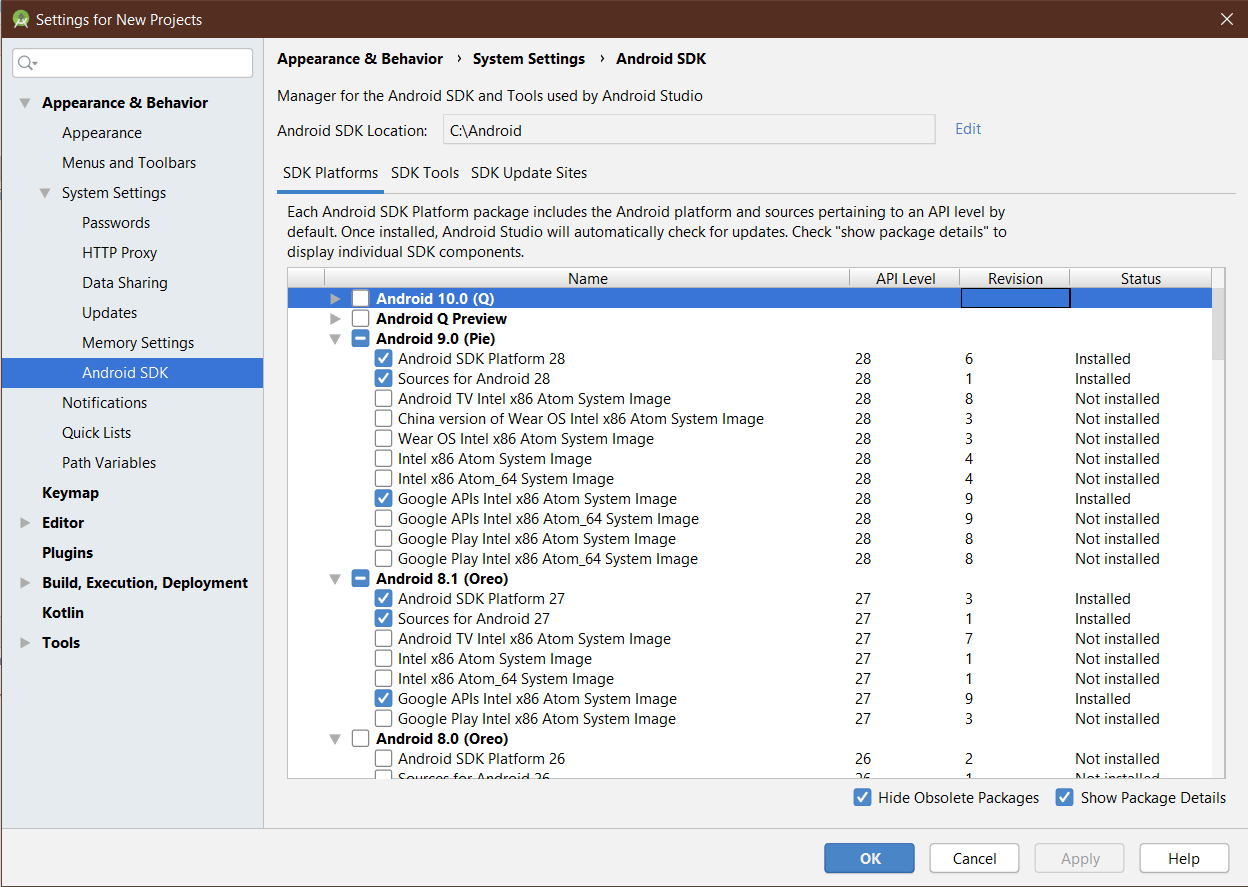
\includegraphics[width=.9\linewidth]{01_sdk_manager.png}
  \caption{SDK manager after installing the required components}
  \label{sdk_manager}
\end{figure}

\section{Question 2}

The process of creation of a virtual device using the \emph{AVD manager} provided by the Android Studio environment involves three steps:

\begin{itemize}

\item The selection of the physical device to be emulated: in this case, the \emph{Pixel 2XL} has been used for both devices;
\item The selection of the system image to be used: in this case, the Oreo (8.1) system image has been chosen for the first device and the Pie (9.0) system image for the second device;
\item The selection of a name for the device and the setting of some advanced parameters, which were left at their default values.

\end{itemize}

After the creation of the two virtual devices, the \emph{AVD manager} shows the screen reported in figure \ref{avd_manager}.

\begin{figure}[H]
  \centering
  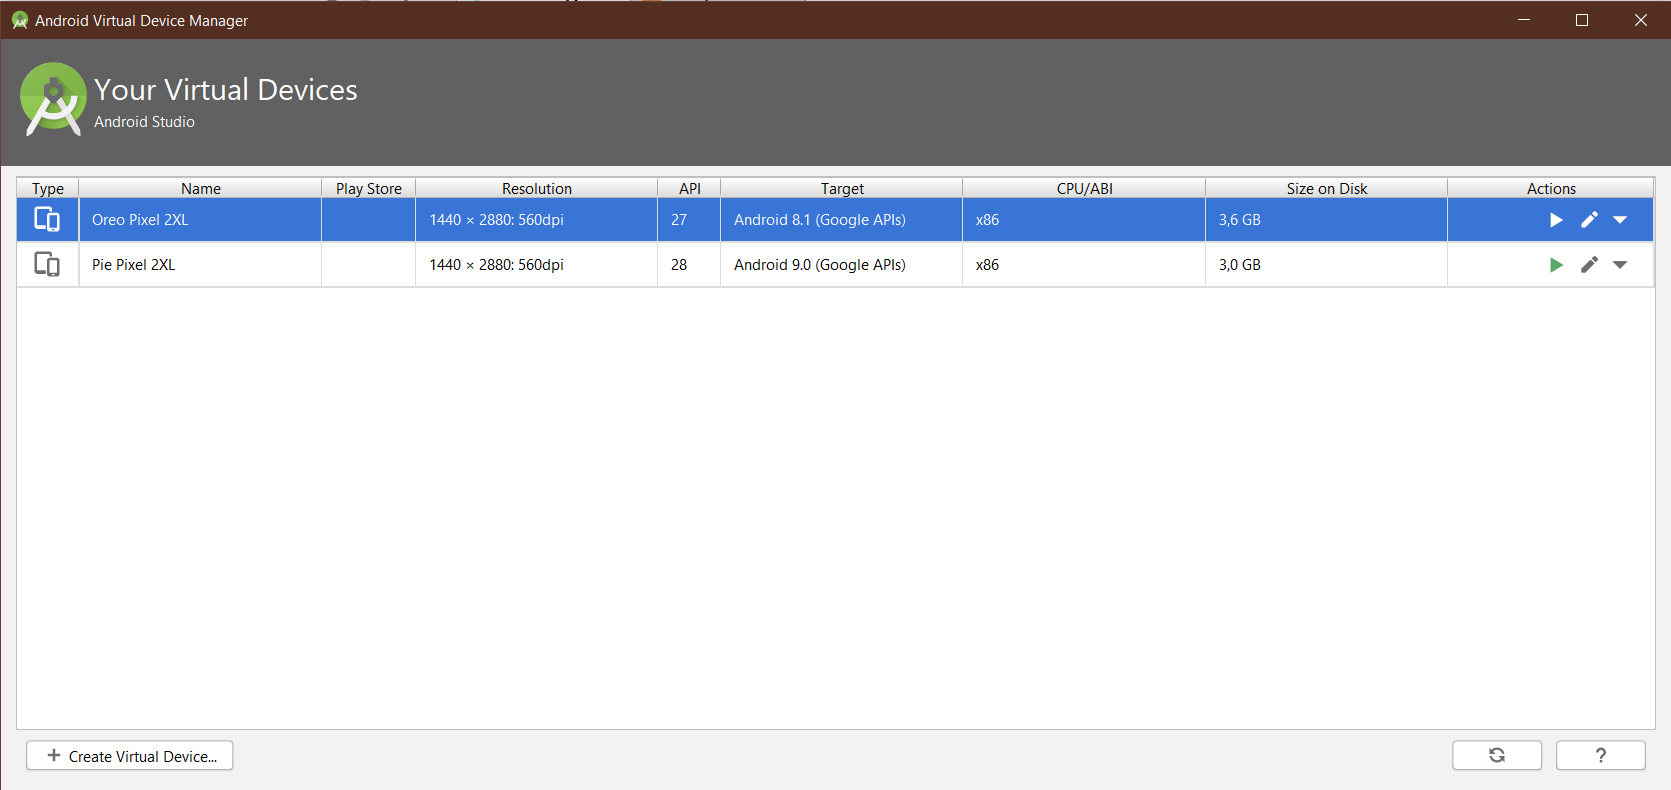
\includegraphics[width=.9\linewidth]{02_avd_manager.png}
  \caption{AVD manager after the creation of the two devices}
  \label{avd_manager}
\end{figure}

The two devices may be started using the opportune action provided by the \emph{AVD manager}; after the boot of the device, the typical Android home screen is shown and it is possible to use the emulator as if it was a real device. The home screen of the two devices running Android 8.1 and 9.0 are shown in figure \ref{running_devices}.

\begin{figure}[H]
  \centering
  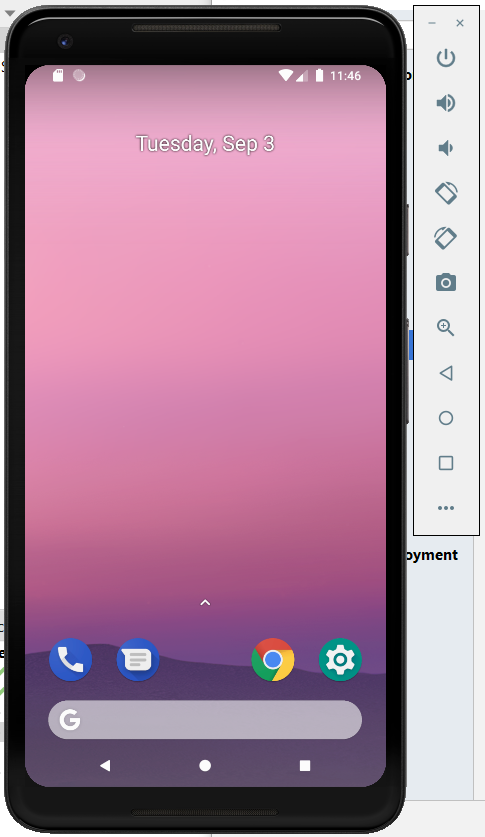
\includegraphics[width=.3\linewidth]{02_oreo_pixel.png}\hfil
  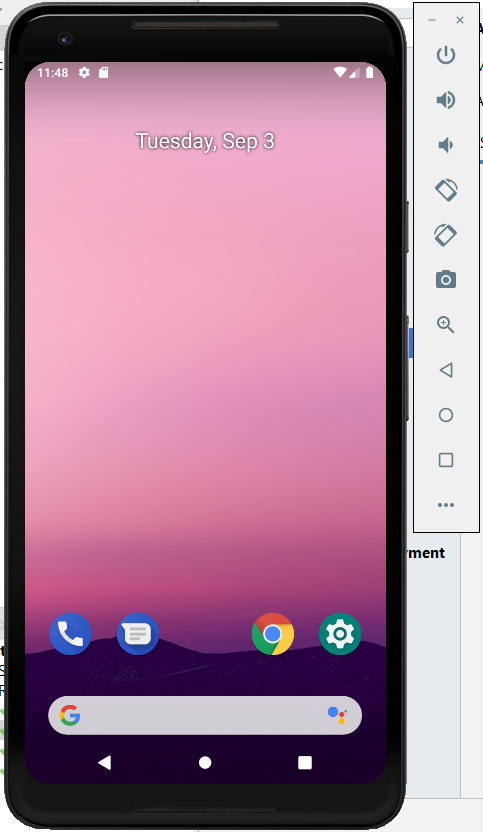
\includegraphics[width=.3\linewidth]{02_pie_pixel.png}
  \caption{The two created devices running in the emulator}
  \label{running_devices}
\end{figure}

\section{Question 3}

In order to obtain the requested message to be printed on screen, the only parameter that has to be changed in the default application as initialized by Android Studio is the \texttt{text} attribute of the \texttt{TextView} component in the \texttt{MainActivity} activity. This can be done in two ways:

\begin{itemize}

\item By manually modifying the layout file associated to the activity containing the \texttt{TextView} component (in this case, it is called \texttt{activity\_main.xml}): it is sufficient to change the value associated to the \texttt{android:text} key inside the \texttt{TextView} block to the desired message;

\item By using the graphical interface provided by Android Studio: after selecting the \texttt{TextView} component, the value of the \texttt{text} attribute can be viewed and edited in the right column, under the \emph{Common Attributes} section, as shown in figure \ref{common_attributes}.

\begin{figure}[H]
  \centering
  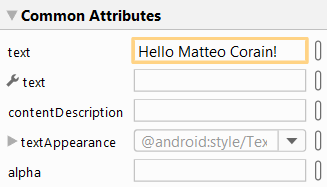
\includegraphics[width=.4\linewidth]{03_attributes.png}
  \caption{Common Attributes section in the Android Studio GUI}
  \label{common_attributes}
\end{figure}

\end{itemize}

At this point, the application is ready to be compiled and sent to a device. In order to do so, it is necessary to:

\begin{itemize}

\item Enable the \emph{USB Debug} option on the device through the \emph{Developer Options};
\item Connect the device to the PC and accept the request of connection;
\item Select the name of the physical device to be used in the navigation bar of Android Studio, as shown in figure \ref{device_debug};

\begin{figure}[H]
  \centering
  
\includegraphics[width=.4\linewidth]{03_device_debug.png}
  \caption{Device selection for application running}
  \label{device_debug}
\end{figure}

\item Build and run the application through the command provided by the IDE.

\end{itemize}

The application consequently runs on the specified device and shows the screen reported in figure \ref{device_run}.

\begin{figure}[H]
  \centering
  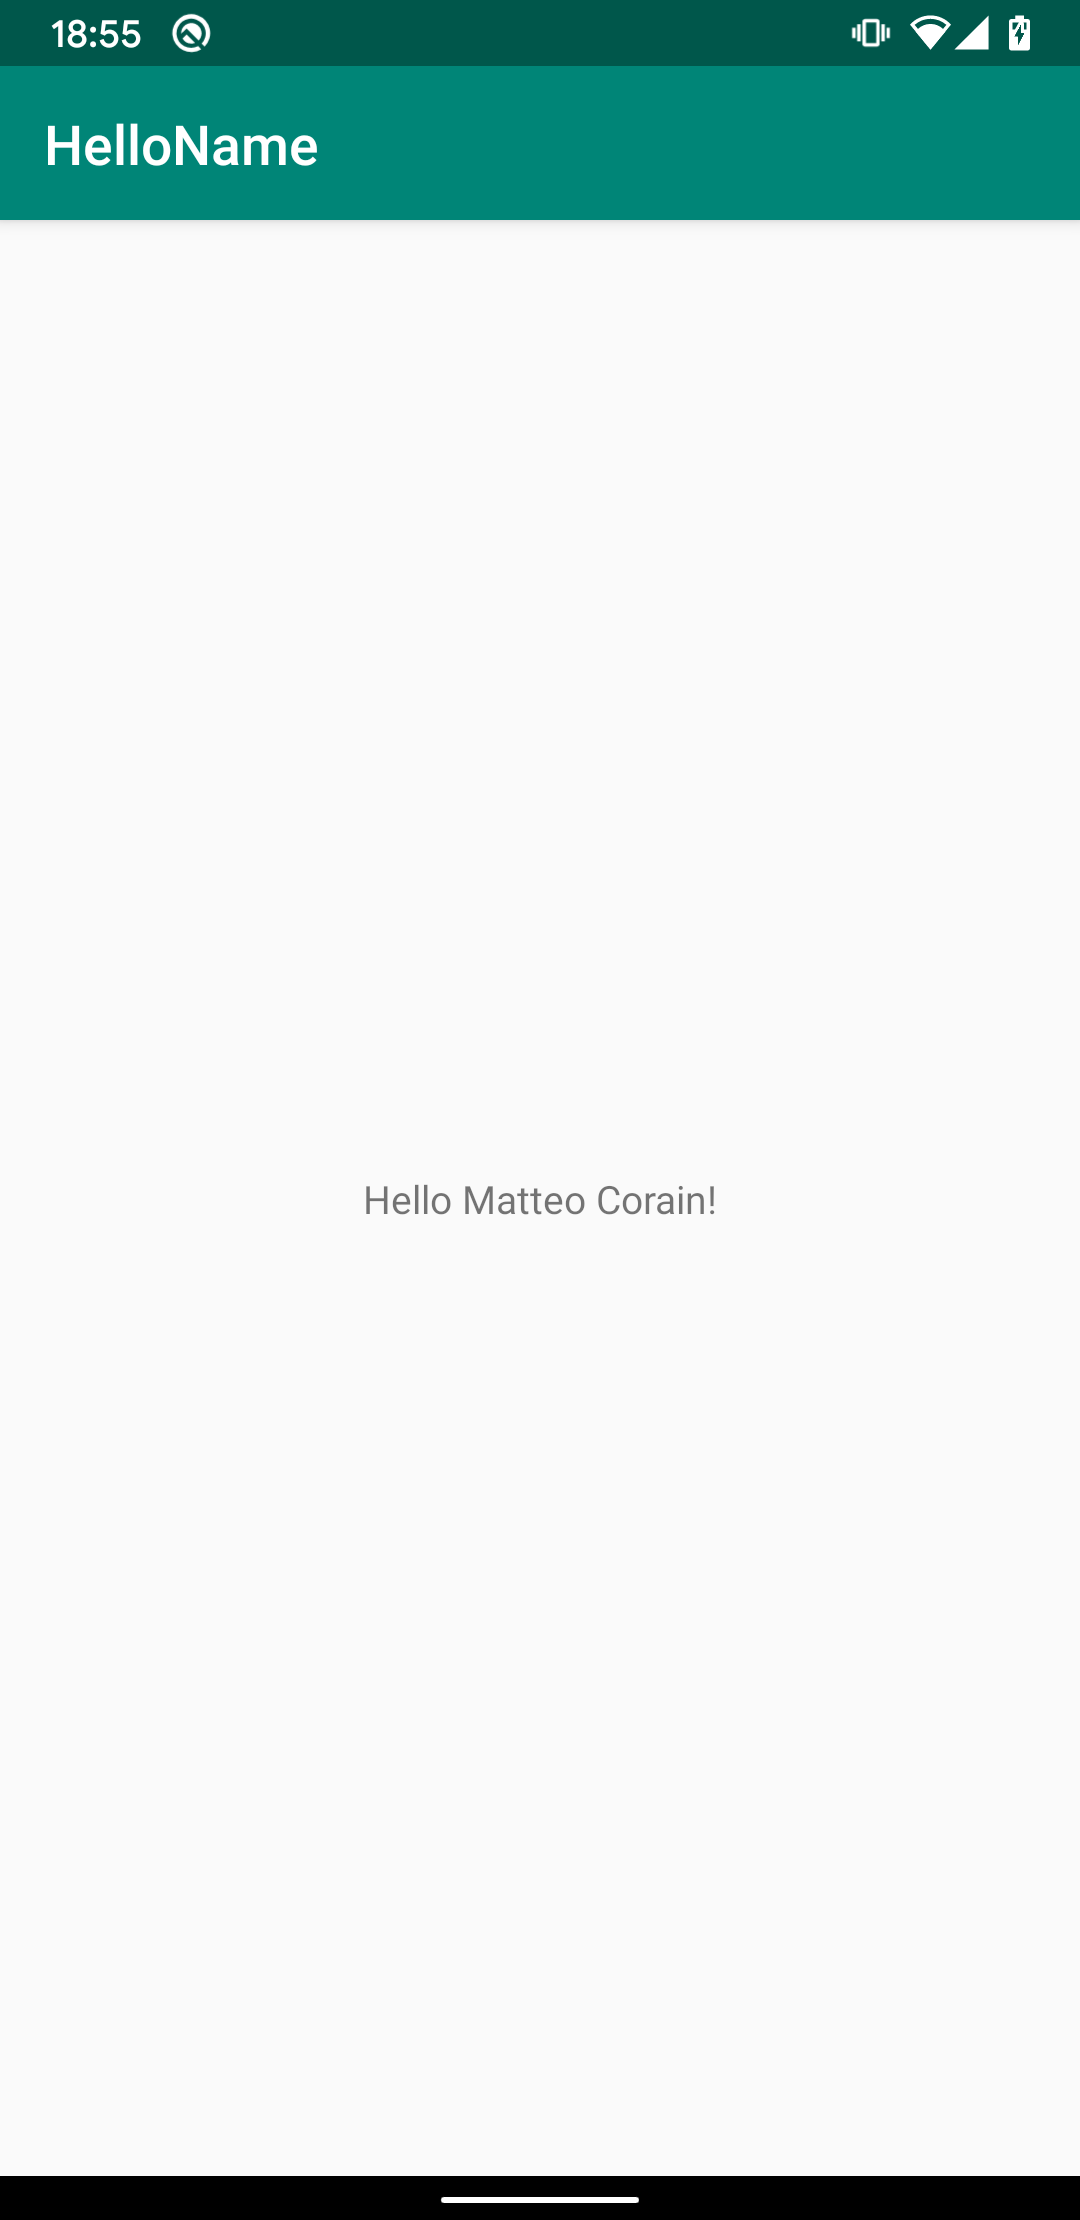
\includegraphics[width=.35\linewidth]{03_device_run.png}
  \caption{Application running on the selected device}
  \label{device_run}
\end{figure}

\section{Question 4}

In order to allow the application to output a \emph{Logcat} statement with a \texttt{INFO} priority level, the static method \texttt{i()} of the \texttt{Log} class has been used. Specifically, the following line has been added to the \texttt{onCreate()} method as provided by Android Studio:

\begin{quote}
\begin{verbatim}
Log.i(TAG, "Matteo Corain was here!");
\end{verbatim}
\end{quote}

Where \texttt{TAG} is a string constant set to \texttt{"MainActivity"}. As an effect, when the application is started on a device, the corresponding line is printed on the \emph{Logcat} tab of Android Studio, as shown in figure \ref{logcat}.

\begin{figure}[H]
  \centering
  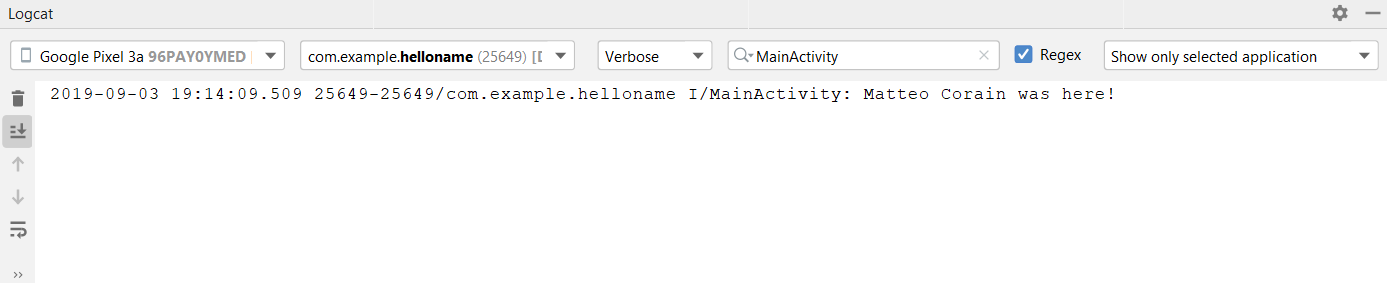
\includegraphics[width=.9\linewidth]{04_logcat.png}
  \caption{Logcat output in Android Studio}
  \label{logcat}
\end{figure}

\end{document}